%  Pt3.tex
% !TeX spellcheck = en_GB
% !TeX root = ProjectRiskManagement.tex
\section{Evaluate \textit{All} the Relevant Implications} \label{s:Evaluate}

%For the evaluate phase of the PUMP approach, in the execution and delivery strategy shaping phase of a project’s lifecycle, explain concisely in your own words what you believe are the key features of a PUMP approach, comparing these features with the PMI PIMBOK approach or any other form of common practice you are familiar with. Your discussion should demonstrate your ability to understand a particular area of the course material in depth, based on selective reading, critical analysis and the case study exercise. Use examples to illustrate your discussion if you wish, and make use of the Transcon case study if you wish, but concentrate on concepts and principles. Build on your Parts 1 and 2 answers, avoiding repetition.

%900 words.

The evaluate phase is the pivotal phase of the PUMP process and plays a critical role in consolidating understanding and controlling PUMP iterations.
The phase involves collating all of the insight and results gained during previous phases into a coherent and comprehensive narrative understanding of the uncertainty involved and the response options available in a clarity efficient manner.
An intuitive understanding of statistical and causal dependence is required to adequately understand the implications of underlying, often-complex relationships.
Following result synthesis, the results must be presented in the most clarity efficient method, usually diagrammatic, to allow interpretation of their practical meaning to ensue.

The phase deliverables may be a simple list of priority sources and responses at early project stages.
This may be developed further to diagnose specific issues and suggested revisions to base plans so that specific sources of risk inefficiency are avoided, and to ensure opportunities are captured.
There are five `modes' of operation of the phase, shown in figure \ref{Figure:Evaluate}.

\begin{figure}[!h]
  \centering
    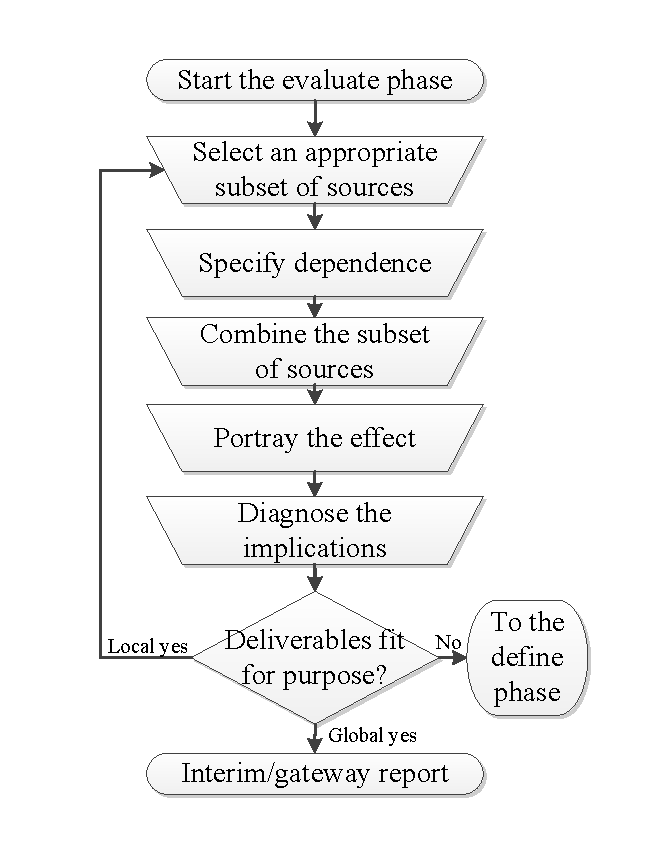
\includegraphics[width = 0.42\textwidth]{./Figures/Evaluate.pdf} 
\caption{Evaluate Phase Process - adapted from \cite{chapman}}
\label{Figure:Evaluate}
\end{figure}

Specifying dependence is an important mode of the phase.
To simplify the approach, many practioners following common practice may assume independence between sources.
This is an extremely dangerous tendency, and any formal analysis based on this assumption on a non-evidential basis should be immediately discounted.
Falsely assuming independence paints an optimistic picture by ignoring the knock-on effects of ignored underlying complexity.
This can be compounded by computational tools aiming to make calculations easier, and by a managerial preference for limited variability. 
Positive dependence is a more reasonable assumption, making a more conservative robust assessment of the impacts. 
In high-clarity contexts, complex statistical and causal dependencies may require more sophisticated modelling approaches to adequately understand the full implications.
The dangers of false underestimation of the impacts is shown in the contrast between independent and positive correlation in figure \ref{}.

\inote{Positive Dependence Figure Here}

Another key mode of the phase is the presentation of results. 
The story that has been developed throughout the analysis must be conveyed in the most clarity efficient manner to be of any practical value to the project organisation.
Sensitivity diagrams are an important tool for conveying and explaining uncertainty.
The common phrase ``a picture is worth a thousand words'' is relevant here.
A sensitivity diagram gives the audience the required information in a non-threatening easy-to-grasp format so that intepretation can take place and issues raised can be resolved.

The sensitivity diagram shown in figure \ref{} shows the collation of NUMBER sources associated with Geotechnical Investigations in preparation for the construction of a power station.
The gap between each curve portrays the effect of the labelled source, so that NUMBER is clearly the most important in this case. The ordering of the sources are important, so that causal and statistical dependence is portrayed.

\inote{Sensitivity diagram 11.5 shown Chapman \& APM}

It may be useful to expand a sensitivity diagram where schedules are concerned. 
Uncertainty can be decomposed through a number of project milestones and contracting activities.
This can be displayed alongside a Gantt chart to portray the schedule implications to the reader.

\inote{Diagram and explanation about gantt sensitivity}

There are also other types of sensitivity diagram which may be useful for presenting uncertainty when there are several different parameters involved. 
One of these is the tornado diagram

\inote{Tornado!!!}

\inote{sensitivity in diagnosis?}

\inote{conclusions!}


